\documentclass{cmspaper}
\usepackage{graphicx}
\begin{document}

%==============================================================================
% title page for few authors

\begin{titlepage}

% select one of the following and type in the proper number:
%   \cmsnote{2008/000}
  \internalnote{2008/000}
%  \conferencereport{2005/000}
   \date{1 April 2008}

  \title{CMS Paper Template - LaTeX version}

  \begin{Authlist}
    A.~Author, B.~Author, C.~Author\Aref{a}
       \Instfoot{cern}{CERN, Geneva, Switzerland}
    D.~Author, E.~Author\Aref{b}, F.~Author
       \Instfoot{ieph}{Institute of Experimental Physics, Hepcity, Wonderland}
  \end{Authlist}

% if needed, use the following:
%\collaboration{Flying Saucers Investigation Group}
%\collaboration{CMS collaboration}

  \Anotfoot{a}{On leave from prison}
  \Anotfoot{b}{Now at the Moon}

  \begin{abstract}
    This is a template written in LaTeX,
    processed with {\it cmspaper.cls} document class.
    It is based on the {\it cernart.cls} and {\it articlet.cls} classes.
    The above information, Title and Abstract, should be readable on any 
    computer and should be searchable on the information server. 
    Therefore if the abstract or the title of your note contains Greek 
    characters and mathematical symbols, please send to the CMS secretariat 
    alternative versions which do not contain such characters.
  \end{abstract} 

% if needed, use the following:
%\conference{Presented at {\it Physics Rumours}, Coconut Island, April 1, 2005}
%\submitted{Submitted to {\it Physics Rumours}}
%\note{Preliminary version}
  
\end{titlepage}

\setcounter{page}{2}%JPP


\section{Introduction}
In CMS the reconstructed objects like electrons, photons, muons, taus, and jets
may have overlap in energy. The multiple counting of any energy fraction must be
avoided in order to obtain optimal energy resolutions of these objects. This is
especially true for the missing transverse energy (MET). The details how the
shared energy is split between two objects will depend on the details of each
analysis. In this note a cross-cleaning package~\cite{package} is discussed,
that is flexible enough to allow the implementation any energy splitting
algorithm between objects. If more than two objects share energy, circular
dependencies may arise. These possible interferences are dealed with, so that
the outcome of cross-cleaned objects does not depend on the order in which the
cleaning algorithms are called.


\section{The Cross-Cleaning-Algorithm Framework}
The cross-cleaning is performed in two steps: First binary cleaners, i.e.
specialized algorithms that clean two collections of objects against eachother,
are called (for example electron-vs.-photon cleaner, muon-vs.-jet cleaner etc.).
These binary cleaners do not apply any corrections on either of the two input
collections, but save the result of the cleaning algorithms in an internal map.
An entry in this map would be the object that should be corrected, the object
that is causing this correction, and finally the information how the object
should be corrected.

In a second step, this temporary buffer map is scanned for possible conflicts.
If the same object {\it A} is causing a correction to object {\it B} but should
be corrected itself because of object {\it C}, than it might happen that after
the correction of {\it A} the correction of {\it B} is no longer necessary or at
least different.

\begin{figure}[hbtp]
  \begin{center}
    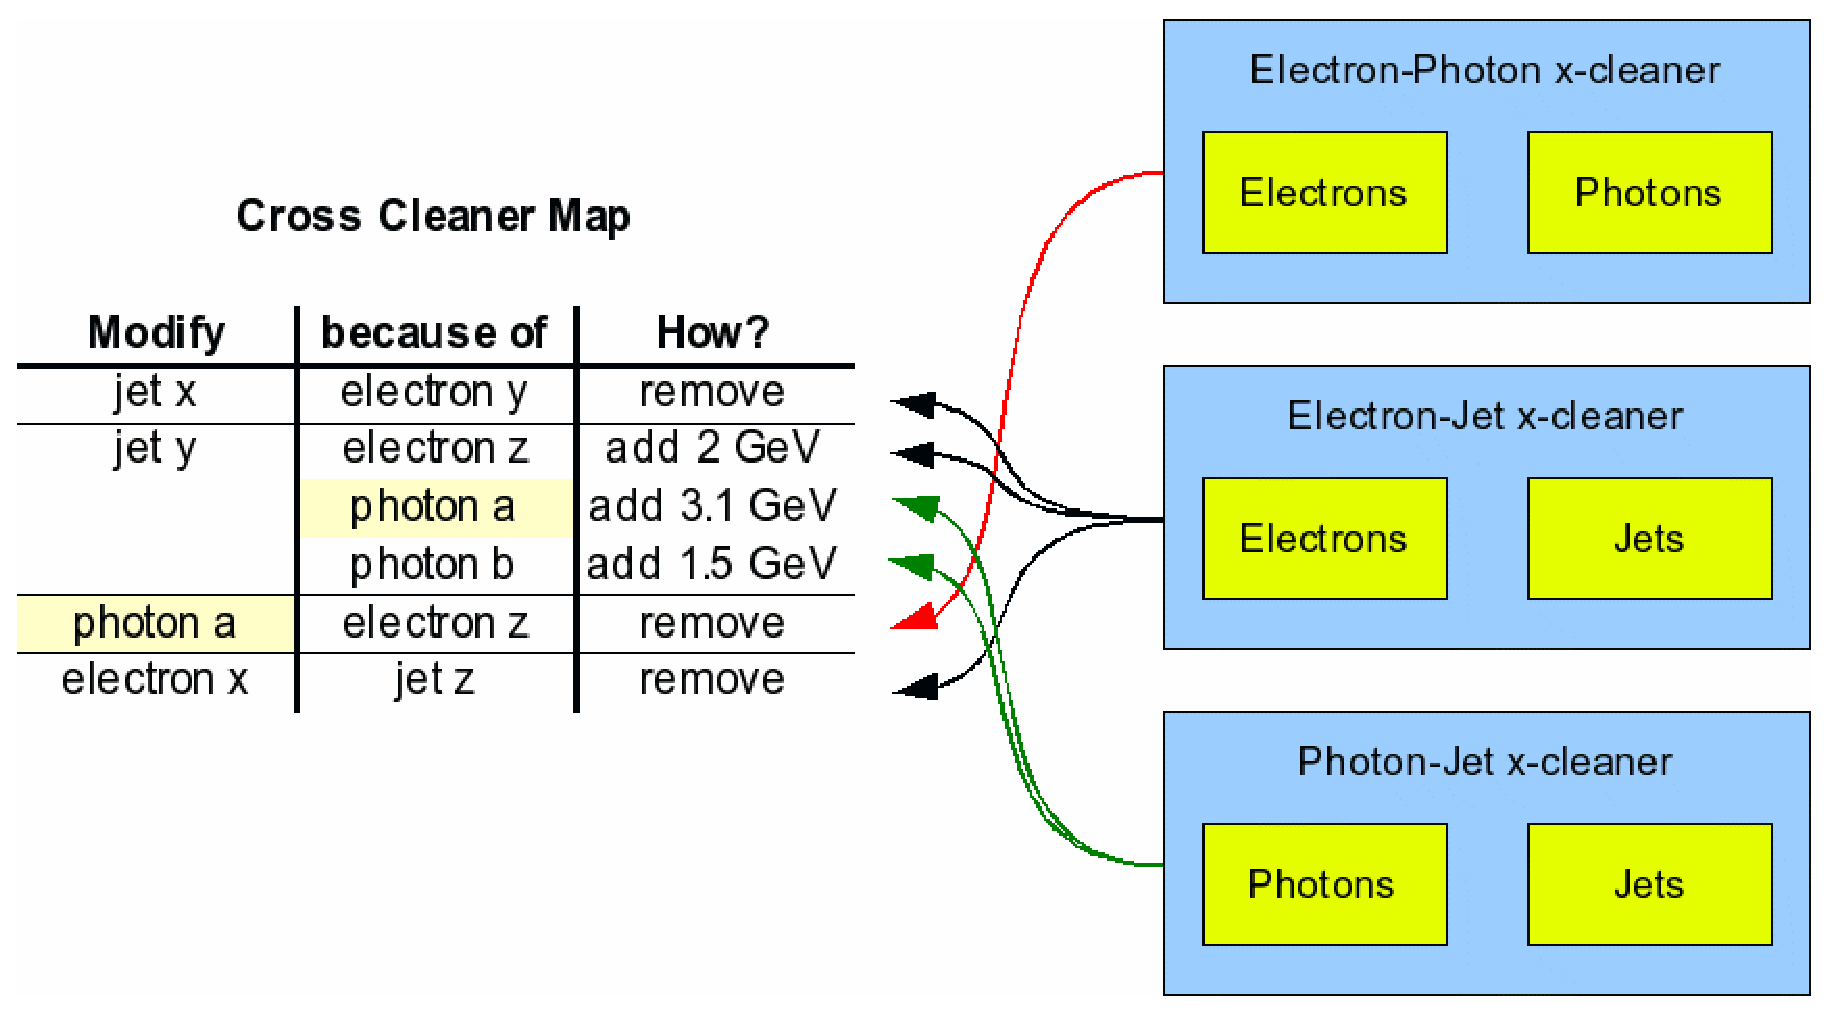
\includegraphics[scale=.4]{CleaningMap.eps}
    \caption{Example Figure inserted by.}
    \label{fig:Cleaning}
  \end{center}
\end{figure}


details,

recalculation of MET

CrossCleanerMap used internaly, Input-Output-Reference Map for external
debugging

\section{Electron - Photon Cleaner}
\subsection{Algorithm}
\subsection{Validation}

\section{Electron - Jet Cleaner}%%Or better: EM-object - jet Cleaner ???
%% \section{Photon - Jet Cleaner}
\subsection{Algorithm}
\subsection{Validation}

\section{Muon - Jet Cleaner}
\subsection{Algorithm}
\subsection{Validation}

\section{Conclusion}


\pagebreak
\begin{thebibliography}{9}
  \bibitem {package} {\bf The CVS code repository},
    \underline{http://cmssw.cvs.cern.ch/cgi-bin/cmssw.cgi/UserCode/SusyAnalysis/PatCrossCleaner/}

  \bibitem {twiki} {\bf The online documentation},
    \underline{https://twiki.cern.ch/twiki/bin/view/CMS/SusyPatCrossCleaner/}
\end{thebibliography}
 
%------------------------------------------------------------------------------

\end{document}
